% encoding: utf8
% !TEX encoding = utf8
% !TeX spellcheck = pl_PL


\documentclass[12pt,a4paper]{article}
\usepackage[margin=0.8in]{geometry}
\usepackage{amsmath}
\usepackage{amssymb}
\usepackage[english,polish]{babel}
\usepackage{cite}
\usepackage{graphicx}
\usepackage{hyperref}
\usepackage[utf8]{inputenc}
\usepackage{listings}
\usepackage{polski}
\usepackage{url}
\usepackage{float}
\usepackage[nottoc]{tocbibind}


\graphicspath{ {./img/} }


\lstset{
	basicstyle=\ttfamily,
	columns=fullflexible,
	frame=single,
	breaklines=true,
	postbreak=\mbox{{$\hookrightarrow$}},
}


\begin{document}
	\title{Pracownia dyplomowa magisterska \\ Sterowanie ramieniem robota w obliczu chwytania przedmiotów}
	\author{Jakub Postępski}
	\maketitle
	
	
	\section{Wprowadzenie}
	Celem tej pracy magisterskiej jest rozwiązanie problemu kompensacji grawitacji w ramieniu robota sterowanym impedancyjnie. Zakłada się nieznany model chwytanego obiektu, znany model ramienia robota oraz nieważkość ramienia robota. Zakładamy dostępność pomiarów z nadgarstkowego czujnika siły i momentu. W trakcie wspomnianej kompensacji grawitacji robot nie powinien tracić swoich zalet związanych z tym typem sterowania. Dodatkowo ramię robota zakończone jest chwytakiem który pozwala na chwytanie przedmiotów.
	
	Środowiskiem badawczym jest robot Velma\cite{velma} (rys. \ref{fig:velma}). Ma on dwa ramiona LWR\cite{lwr} sterowane impedancyjnie. Posiadają wbudowaną kompensację grawitacji własnej masy. Na ich końcach znajdują się chwytaki Barretta oraz nadgarstkowe czujniki FTS.
	
	\begin{figure}[H]
		\centering
		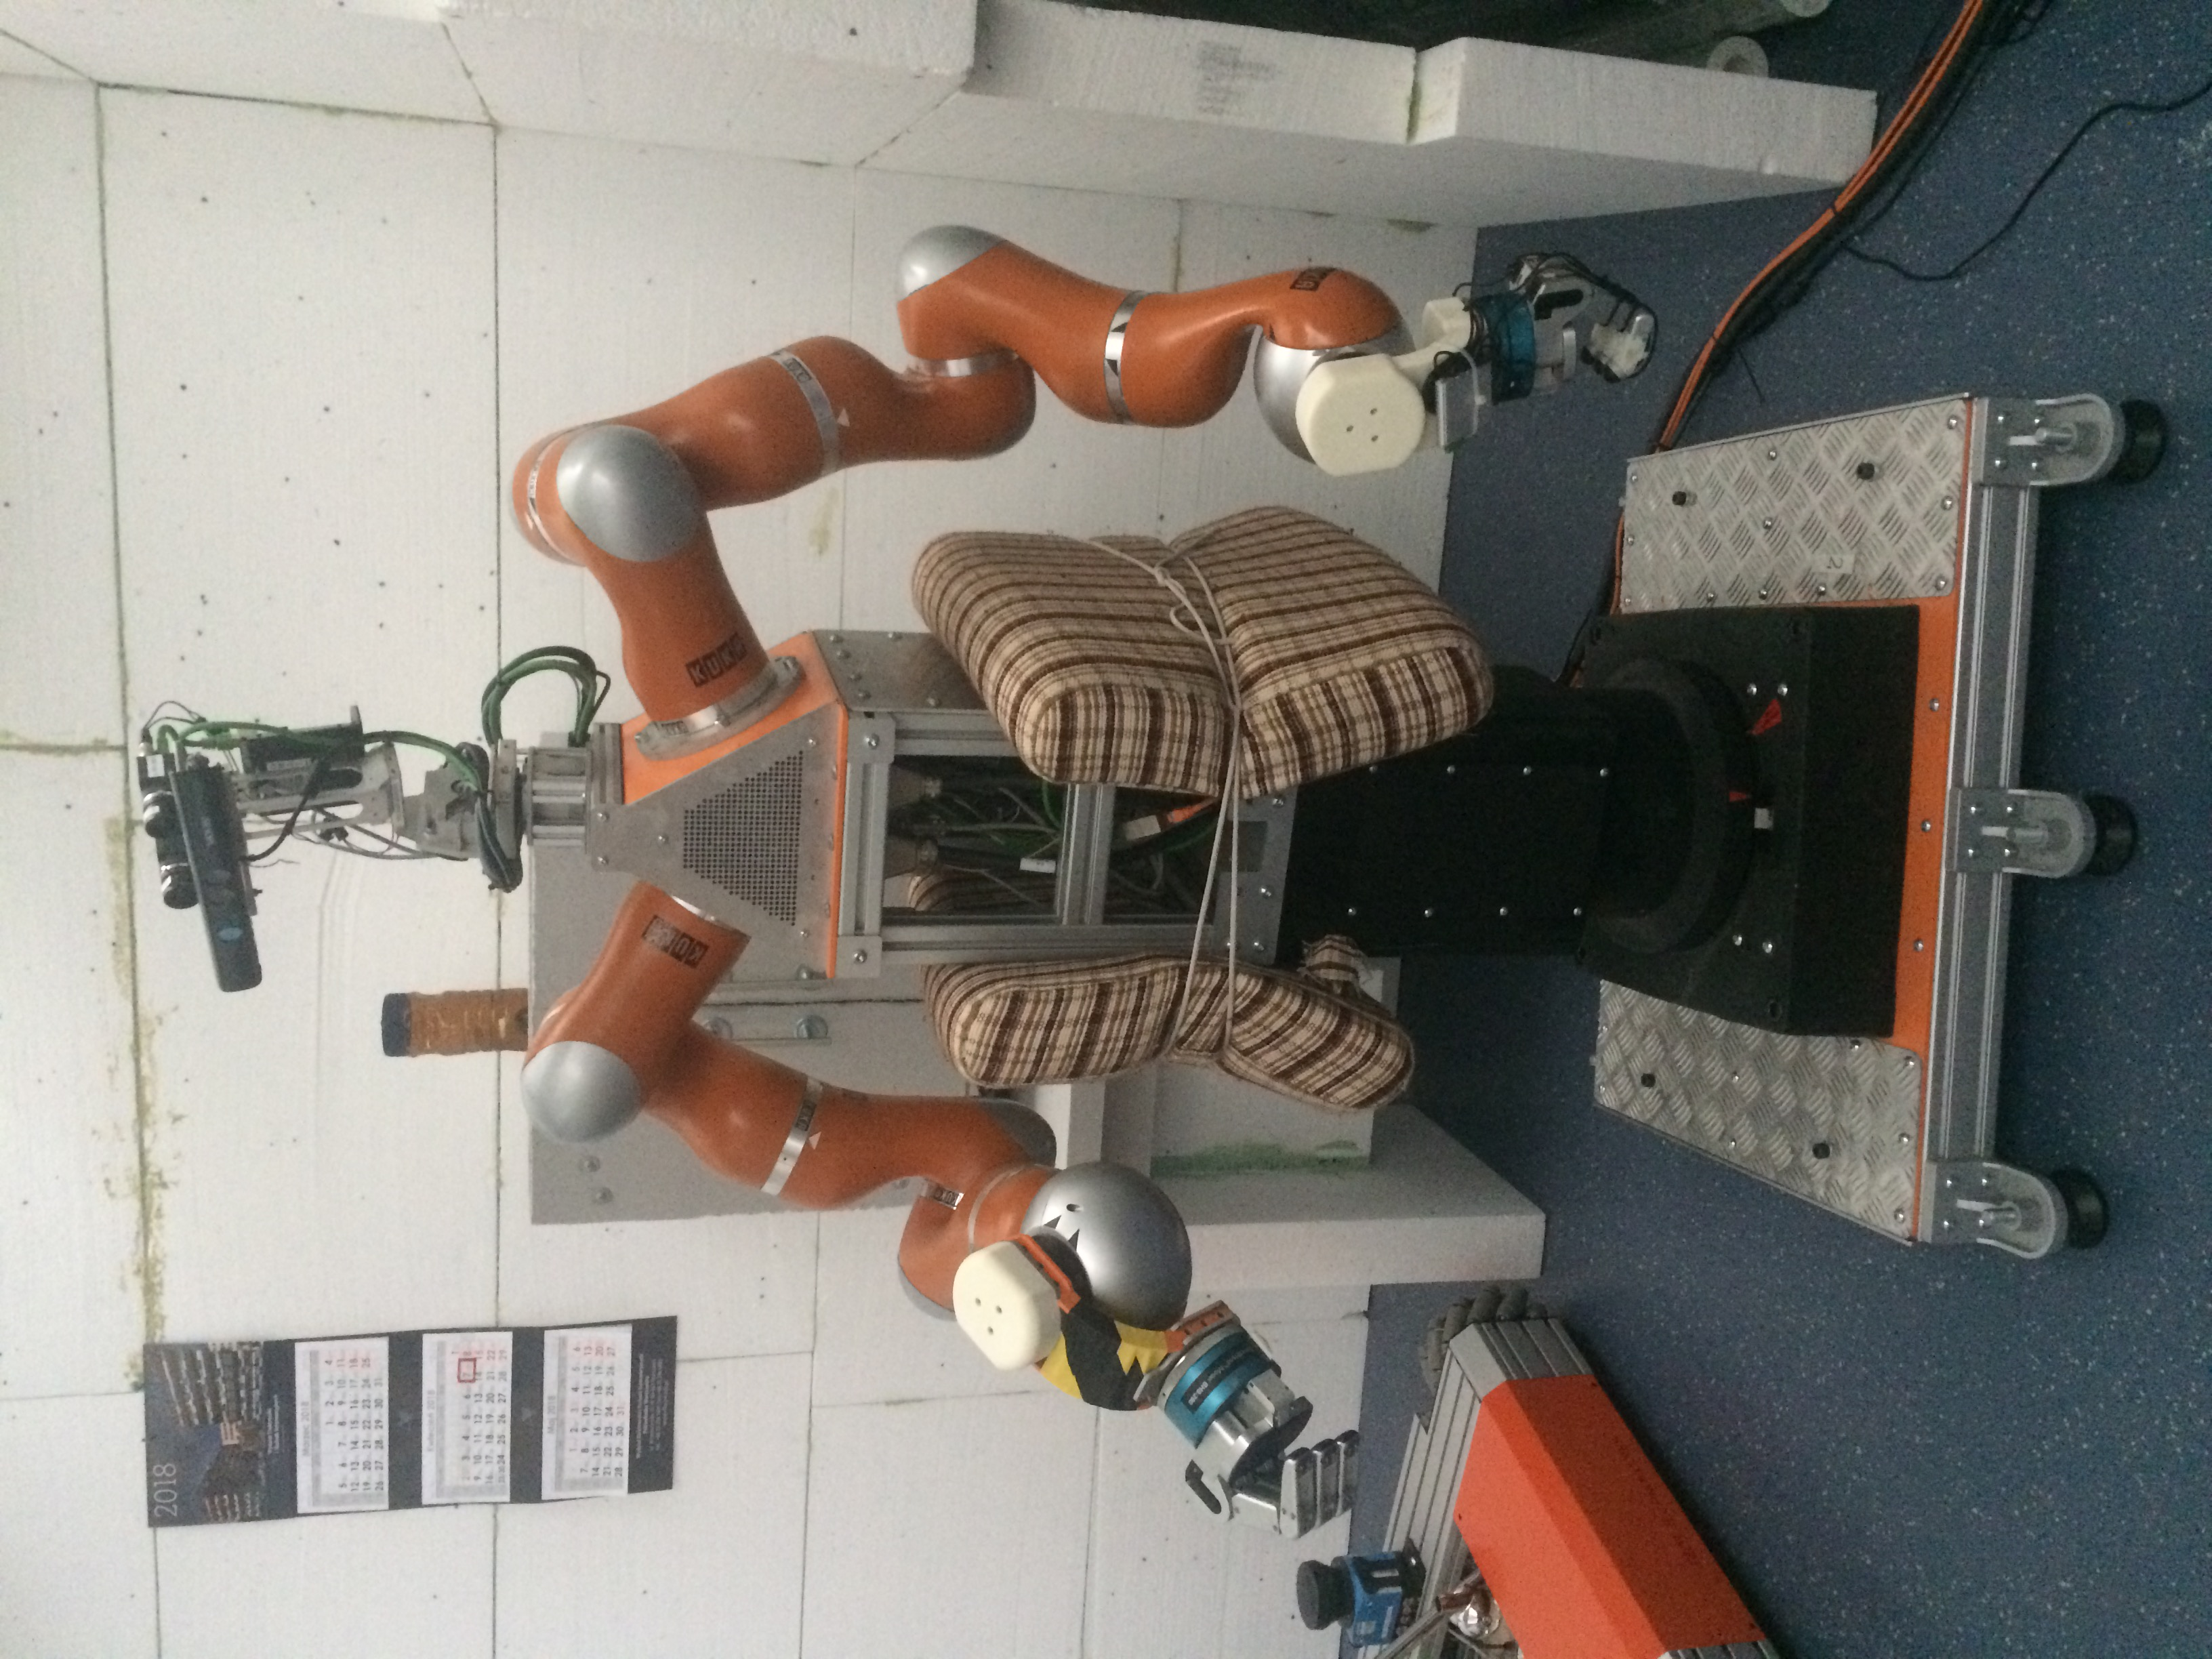
\includegraphics[scale=0.05, angle =-90]{velma}
		\caption{Robot usługowy Velma}
		\label{fig:velma}
	\end{figure}
	
	System sterowania o twardych ograniczeniach czasowych pracuje z częstotliwością 500 Hz. Struktura oprogramowania (rys. \ref{fig:agenty}) została stworzona w oparciu o teorię agentową. Agent \textbf{velma\_core\_cs} jest odpowiedzialny za kontrolę zadań związanych z manipulacją w przestrzeni operacyjnej i konfiguracyjnej robota poprzez kontrolę efektorów i receptorów robota. Agent \textbf{velma\_ros\_interface} służy do kontroli i interpretacji zadań zleconych przez użytkownika poprzez zarządzanie agentem \textbf{velma\_core\_cs}. Oprogramowanie agenta \textbf{velma\_core\_cs} jest wykonane przy wykorzystaniu struktury ramowej Orocos, natomiast agenta \textbf{velma\_ros\_interface} przy użyciu struktury ramowej ROS. Dostępny jest też symulator robota pisany w przy wykorzystaniu Gazebo. Do obserwowania pracy poszczególnych komponentów systemu służy narzędzie rqt\_agent.
	
	\begin{figure}[H]
		\centering
		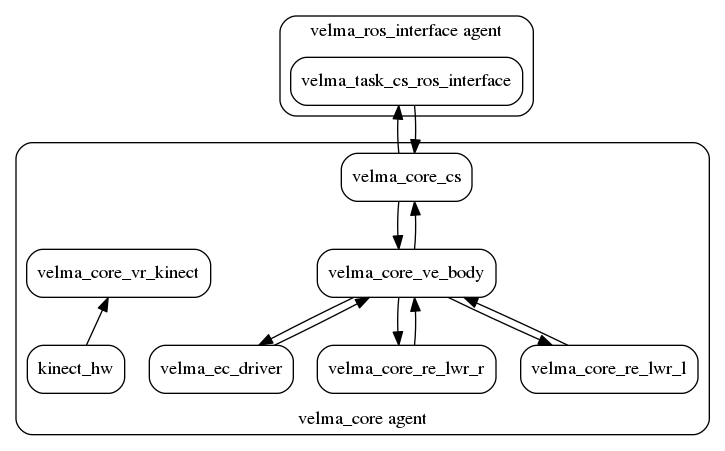
\includegraphics[width=0.8\linewidth]{agenty}
		\caption{Agentowa struktura oprogramowania \cite{velma}}
		\label{fig:agenty}
	\end{figure}
	
	\section{Prace badawcze}
	\subsection{Artykuły}
	Artykuł \cite{impedance} pozwala na zrozumienie podstaw sterowania impendancyjnego dla ramion robotów. Artykuły \cite{gravity1} i \cite{gravity2} przedstawiają przykładowe rozwiązania problemu kompensacji grawitacji.
	
	Na wykładach z Teorii sterowania można uzyskać wiedzę na temat podstawowych struktur sterowania. Poruszane są problemy systemów z czasem dyskretnym. Omawiane są problemy konstrukcji optymalnych estymatorów regulatorów i obserwatorów. Jeden z wykładów poświęcony został regulacji adaptacyjnej. Omawiane są zagadnienia niwelowania szumów znajdujących się w układzie. 	Na przedmiocie Algorytmy i metody optymalizacji poruszana jest tematyka optymalizacji funkcji liniowych i nieliniowych z ograniczeniami. Omawiany jest problem sprowadzania optymalizacji funkcji nieliniowej i niewypukłej do prostszych postaci. Prezentowane są szybkie algorytmy optymalizacji funkcji kwadratowych. W ramach wykładów z  Modelowania i sterowania robotów omawiane są zagadnienia opisu kinematyki i dynamiki robotów. Na przedmiocie Inteligentne systemy robotyczne omawiane są zagadnienia teorii agentowej i zastosowania tej teorii w robotyce.
	
	Uczęszczanie na wykłady oraz czytanie artykułów pozwoliło na wyrobienie ogólnego poglądu na przedstawiony problem. Szczególnie istotne była zdobyta wiedza na temat optymalnych regulatorów i obserwatorów. Ważne okazały się też metody optymalizacji ponieważ mogą pozwolić na sprawną implementację wymienionych narzędzi.
	
	
	\subsection{Sformalizowanie problemu}
	Należy skompensować siłę grawitacji w układzie stawu obrotowego sterowanego impedancyjnie. Rozwiązaniem jest określenie masy a następnie dodanie odpowiednich sił do układu w celu kompensacji siły grawitacji.
	
	Obiektem jest układ wahadła sterowanego prawem sterowania impedancyjnego (rys. \ref{fig:2d}). Na końcu nieważkiego ramienia $r$ zawieszona jest punktowa masa $m$ której grawitację należy skompensować. Algorytm sterowania symuluje sprężynę oraz amortyzator w osi obrotu wahadła i można do niego dodać moment $u$.  Przyjmujemy że dla użytkownika dostępne są pomiary położenia $q$, prędkości $\dot{q}$, przyspieszenia $\ddot{q}$. Dodatkowo przyjmujemy, że w osi obrotu znajduje się czujnik FTS odczytujący siłę $F$ i moment siły $\tau$.
	
	Układ z inercją $I$ możemy opisać przy pomocy równania:
	\begin{equation}
	\label{eq:intro}
	\tau = I\ddot{q} = mr^2\ddot{q} = kq + d\dot{q} + mgr\cos{(q)} + Iu
	\end{equation}
	
	Model obiektu można opisać układem równań różniczkowych:
	\label{eq:intro2}
	\begin{equation}
	\begin{bmatrix}
	\dot{q} \\
	\ddot{q}
	\end{bmatrix}
	=
	\begin{bmatrix}
	0 & 1 \\
	\frac{k}{I} & \frac{d}{\tau_u}
	\end{bmatrix}
	\begin{bmatrix}
	q \\
	\dot{q}
	\end{bmatrix}
	+
	\begin{bmatrix}
	0 \\
	\frac{1}{I}
	\end{bmatrix}
	(mgr\cos{(q)} + \tau_u)
	\end{equation}
	
	gdzie:
	\begin{itemize}
		\item $q$ - kąt obrotu [$rad$]
		\item $k$ - sztywność
		\item $b$ - tłumienie
		\item $m$ - masa przedmiotu [$kg$]
		\item $g$ - przyspieszenie ziemskie [$\frac{m}{s^2}$]
		\item $\tau_u$ - moment dodawany w celu kompensacji grawitacji przedmiotu [$Nm$]
	\end{itemize}
	
	Układ możemy więc zapisać w standardowej postaci
	\begin{equation}
	\dot{q} = \textbf{A}q + \textbf{B}u(t)
	\end{equation}
	gdzie:
	\begin{equation}
	\mathbf{A} = 	\begin{bmatrix}
	0 & 1 \\
	\frac{k}{I} & \frac{d}{I}
	\end{bmatrix}
	\end{equation}
	oraz:
	\begin{equation}
	\mathbf{B} = \begin{bmatrix}
	0 \\
	1
	\end{bmatrix}
	\end{equation}
	
	Siła działająca na układ jest sumą siły grawitacji i siły odśrodkowej układu.
	Siłę grawitacji możemy opisać wzorem:
	\begin{equation}
	F_g = mg
	\end{equation}
	a siłę odśrodkową odpowiednio w osi $X$ oraz $Y$ wzorami:
	\begin{equation}
	F_{ox} =  \cos{(q)}m\dot{q}^2 r
	\end{equation}
	\begin{equation}
	F_{oy} =  \sin{(q)}m\dot{q}^2 r
	\end{equation}
	
	
	Dlatego odczyty czujnika w dwóch osiach możemy opisać wzorami:
	
	\begin{equation}
	F_x = F_{ox} = \cos{(q)}m\dot{q}^2 r
	\end{equation}
	
	\begin{equation}
	\label{eq:fy}
	F_y = F_g + F_{oy} = mg + \sin{(q)}m\dot{q}^2 r
	\end{equation}
	
	
	\subsection{Dyskretyzacja układu}
	Po zdyskretyzowaniu metodami ZOH z okresem próbkowania $T$ otrzymujemy układ:
	\begin{equation}
	q(t+1) = \mathbf{A_d}q(t) + \mathbf{B}_du(t)
	\label{eq:dyskretny}
	\end{equation}
	
	Dyskretyzację odczytów FTS  oraz innych równań można przeprowadzić korzystając z dyskretyzacji metodą Eulera ($\dot{q} \approx \frac{q(t)-q(t-1)}{T}$).
	
	\begin{equation}
	F_{dx}(t) = \cos{(q)}m(\frac{q(t)-q(t-1)}{T})^2 r
	\end{equation}
	\begin{equation}
	F_{dy}(t) = mg + \sin{(q)}m(\frac{q(t)-q(t-1)}{T})^2 r
	\end{equation}
	
	oraz z równania \ref{eq:intro}
	\begin{equation}
	\tau(t) = kq(t) + d\frac{q(t)-q(t-1)}{T} + Iu + \cos(q)mg
	\end{equation}
	
	Podobnie można dyskretyzować inne równania i w dalszej części raportu zastosowanie metody nie będzie pokazywane wprost. We wszystkich symulacjach przedstawionych dalej użyto dyskretnych wersji przedstawionych równań.
	
	\subsection{Estymacja nieznanych parametrów}
	W celu skompensowania grawitacji zawieszonej masy należy poznać parametry opisujące tę masę. Uznano że do opisu wystarczą typowe i powszechnie używane zmienne. W opisywanym układzie nie są znane takie wielkości jak inercja, masa oraz środek ciężkości.
	
	Przy założeniu, że masa jest punktowa wiemy że inercję tej masy opisuje zależność
	\begin{equation}
	I = mr^2
	\end{equation}
	W trakcie opisu metod estymacji parametrów starano się w miarę możliwości nie korzystać z tej zależności. Dzięki takiemu podejściu w przyszłości będzie można wykorzystać znalezione metody w celu estymacji mas niepunktowych o nierównomiernym rozkładzie.
	
	Posiadając estymację promienia $r$ i wykorzystując pozycję $q$ jesteśmy w wstanie określić pozycję zawieszonej w układzie masy i jej środek ciężkości.
	
	
	\subsection{Estymacja masy przy wykorzystaniu FTS}
	\label{sec:ftsods}
	Korzystając z równania \ref{eq:fy} można opisać siły działające na czujnik w osi $Y$ w chwili $i$ jako:
	\begin{equation}
	F_{yi}  = m(g + \dot{q_i}^2r\sin{(q_i)})
	\end{equation}
	
	Zakładając błędy odczytu $e$ dostajemy próbkę postaci:
	\begin{equation}
	\hat{F_{yi}}+e_i  = F_{yi}
	\end{equation}
	
	Posiadając $n$ próbek możemy więc sformułować zadanie optymalizacji nieliniowej z parametrami $m$ oraz $r$ takie że:
	\begin{equation}
	\begin{aligned}
	& \underset{m, r}{\text{min}}
	& & \sum_{i = 1}^{n} || e_i || = \sum_{i = 1}^{n} || \hat{F_{yi}} - F_{yi} || \\
	& \text{przy ograniczeniach}
	& & F_{yi} = m(g + \dot{q_i}^2r\sin{(q_i)}), \; i = 1, \ldots, n.
	\end{aligned}
	\end{equation}
	
	Analogicznie można rozwiązać problem estymacji inercji $I$ wykorzystując równanie \ref{eq:intro} i sformułować zadanie optymalizacji:
	\begin{equation}
	\begin{aligned}
	& \underset{I}{\text{min}}
	& & \sum_{i = 1}^{n} || e_i || = \sum_{i = 1}^{n} || \hat{\tau_{i}} - \tau_{i} || \\
	& \text{przy ograniczeniach}
	& & \tau_{i} = I\ddot{q_i}^2, \; i = 1, \ldots, n.
	\end{aligned}
	\end{equation}
	
	\subsection{Estymacja inercji z macierzy układu}
	\label{sec:pos}
	Ponieważ macierz $\mathbf{B}$ ma tylko jeden wyraz różny od zera $\mathbf{B_d}$ jest uzyskiwana w prosty sposób i można przyjąć że:
	\begin{equation}
	\mathbf{B_d} \approx \mathbf{B}T
	\end{equation}
	Przekształcając równanie \ref{eq:dyskretny} i stosując pseudoinwersję macierzy otrzymujemy równanie macierzowe:
	\begin{equation}
	\mathbf{A_d} = (X(t+1) - \mathbf{B}_du(t))(X(t))^{pinv}
	\label{eq:pinv}
	\end{equation}
	przy założeniu $n$ ostatnich próbek zmiennych stanów układu
	\begin{equation}
	X(t) = 	\begin{bmatrix}
	x(t) & x(t-1)  & ... & x(t-n)
	\end{bmatrix}
	\label{eq:xk}
	\end{equation}
	
	Po obliczeniu estymacji $\mathbf{A_d}$ metodą ZOH wyliczamy estymację macierzy $\mathbf{A}$ otrzymując macierz
	\begin{equation}
	\mathbf{\hat{A}} = 	\begin{bmatrix}
	a_{11} & a_{12}\\
	a_{21} & a_{22}
	\end{bmatrix}
	\end{equation}
	Po przyrównaniu jej do macierzy $\mathbf{A}$ możemy wyliczyć inercję z równań:
	\begin{equation}
	\hat{I_1} = \frac{-k}{a_{21}}
	\end{equation}
	\begin{equation}
	\hat{I_2} = \frac{-b}{a_{22}}
	\end{equation}
	
	i ostatecznie przyjąć estymację:
	\begin{equation}
	\hat{I} = \frac{\hat{I_1}+\hat{I_2}}{2}
	\end{equation}
	
	
	Metoda nie pozwala na uzyskanie wszystkich parametrów lecz w przypadku braku czujnika FTS lub uzyskania z niego zaszumionych odczytów można uzyskać tą metodą zadowalające wyniki.
	
	\subsection{Kompensacja grawitacji}
	Kompensacja polega na dodaniu do układu momentu siły który przeciwdziała sile grawitacji masy. Z równania \ref{eq:intro2} wynika postać sterowania $u$ kompensującego siłę grawitacji. Ponieważ zależy nam na tym aby pozbyć się członu związanego z macierzą $\mathbf{B}$
	\begin{equation}
	\begin{bmatrix}
	0 \\
	1
	\end{bmatrix}
	(\frac{mgr\cos{(q)}}{I} + u) = 	\begin{bmatrix}
	0 \\
	0
	\end{bmatrix}
	\end{equation}
	możemy przyjąć sterowanie:
	\begin{equation}
	u_s(t) = -\frac{mgr\cos{(q(t))}}{I}
	\end{equation}
	Masę $m$, promień $r$ oraz inercję $I$ uzyskujemy z estymacji przedstawionych w sekcji \ref{sec:ftsods}.
	
	
	Algorytm kompensacji nie powinien wprowadzać gwałtownych zmian w prezentowanym układzie więc sterowanie kompensujące wpływ grawitacji jest załączany stopniowo. W celu uzyskania takiego efektu sterowanie jest mnożone przez odpowiednią funkcję trapezową. Dla czasu $t_p$ początku załączania algorytmu i $t_k$ końca załączania mamy:
	\begin{equation}
	u(t) = \min{(\frac{\max{( t - t_p, 0)}}{t_k-t_p}, 1)}u_s(t)
	\end{equation}
	
	
	
	\begin{figure}[H]
		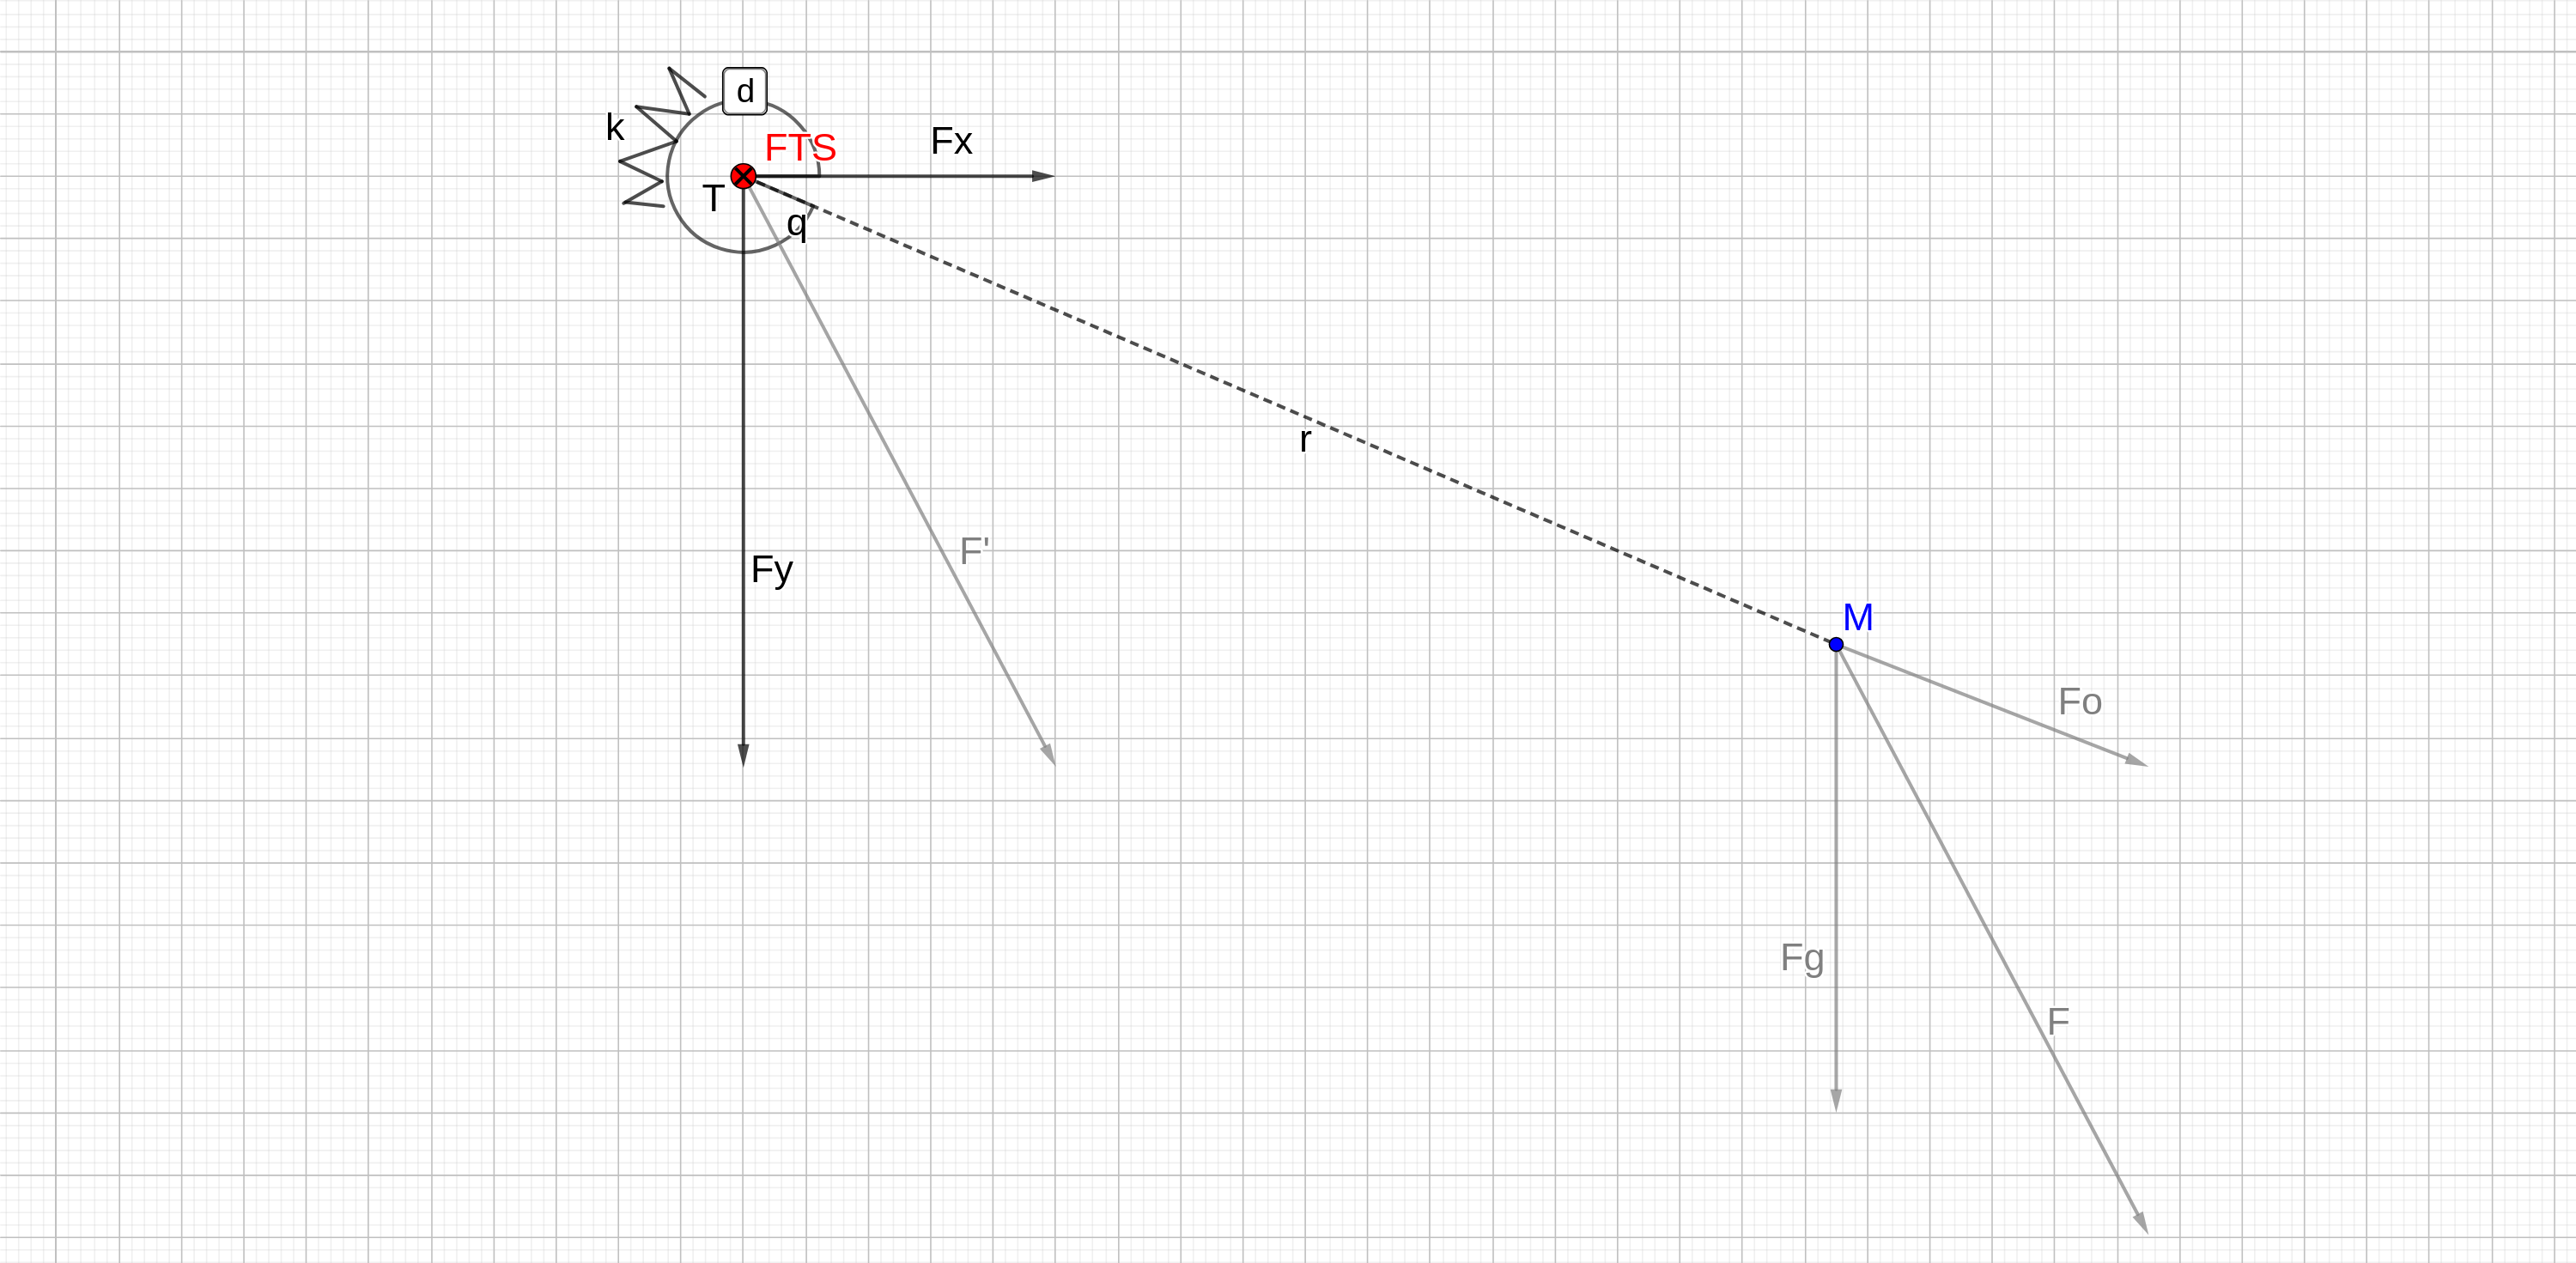
\includegraphics[width=0.99\linewidth]{2d}
		\centering
		\caption{Schemat badanego układu. Kolorem niebieskim zaznaczono masę $m$ zawieszoną na ramieniu $r$. Kolorem czerwonym zaznaczono punkt mocowania ramienie i umiejscowienia czujnika FTS. Kolorem czarnym pokazano siły odczytywane z czujnika sił, moment siły $\tau$, pozycję $q$ sprężynę $k$ oraz amortyzator $d$. Kolorem szarym zaznaczono rzeczywiste siły układu.}
		\label{fig:2d}
	\end{figure}
	
	
	\section{Modyfikacja oprogramowania robota}
	Implementacja praw sterowania znajduje się w podsystemie sterowania agenta \textbf{velma\_core\_cs} \cite{velma}. Zdecydowano się zmianę trybu pracy \textbf{cart\_imp} odpowiedzialnego za sterowanie impedancyjne w przestrzeni konfiguracyjnej. Odpowiedzialny za to jest komponent \textbf{cart\_imp}. Dodano do niego nowe wejście na które można podać dodatkowy moment siły uwzględniany w każdym kroku sterowania. W celu uzyskania odczytów z czujników FTS zmodyfikowano podsystem wirtualnego receptora, tak aby przekazywał odczyty do podsytemu sterowania. Do podsystemu sterowania dodano nowy komponent \textbf{gravity\_compensation} który odbiera odczyty z czujników FTS i na swoje wyjście przekazuje moment sił który należy uwzględnić w prawie sterowania. Komponent będzie dalej modyfikowany.
	
	
	

	\section{Podsumowanie}
	W ramach dotychczasowych prac przedstawiono przeprowadzone badania nad zagadnieniem. Dodatkowo przygotowano symulator środowiska badawczego do implementacji i testowania przedstawionych algorytmów. Do wykonania pozostała praktyczna implementacja rozwiązania oraz testy.
	
	\bibliographystyle{unsrt}
	\bibliography{bibliography}
	
\end{document}



